\documentclass[12pt]{article}

% Imported Packages
%------------------------------------------------------------------------------
\usepackage{placeins}
\usepackage{amssymb}
\usepackage{amstext}
\usepackage{amsthm}
\usepackage{amsmath}
\usepackage{enumerate}
\usepackage{fancyhdr}
\usepackage[margin=1in]{geometry}
\usepackage{graphicx}
\usepackage{extarrows}
\usepackage{setspace}
\usepackage[utf8]{inputenc}
%------------------------------------------------------------------------------

% Header and Footer
%------------------------------------------------------------------------------
\pagestyle{plain}
\renewcommand\headrulewidth{0.4pt}
\renewcommand\footrulewidth{0.4pt}
%------------------------------------------------------------------------------

% Title Details
%------------------------------------------------------------------------------
\title{Large System Design\\
	\large Carspot for SE 3A04, Tutorial 2}
    \author{
         Yasaswi Gopalakrishnan\\ \newline
         \and
         Sharon Platkin \\ \newline
         \and
         Abhijit Singh Dhoat\\ \newline
         \and
         Joseph Cole Huot\\ \newline
         \and
         David Eric Hemms\\ \newline
         \and
         Yuchen Liu\\ \newline
    }
    \date{Monday March 28th, 2016}
% Document
%------------------------------------------------------------------------------
\begin{document}

\maketitle
\newpage
\tableofcontents
\listoftables
\newpage

\section{Introduction}
\label{sec:introduction}
% Begin Section

\subsection{Purpose}
\label{sub:purpose}
% Begin SubSection

The purpose of this document is to provide an outline of the entire system of the android application. The diagrams used in this document identify all main elements and components of the system. The intended audiences for this document are software engineers who intended to work on 3A04 android application project and their instructional staff. The document may be edited if any changes took place on the software requirements specification document.

% End SubSection

\subsection{System Description}
\label{sub:system_description}
% Begin SubSection
The system will be made available to the general public through the Google Play Store on the Android Operating System. Users will download and use the app to identify cars they spot in their day to day lives. 

The user will be prompted by the system to pick from a set of categories they recognize. They will pick 3 of the these: car type, a logo, number of passengers or origin. The system will then search based on the information the user provides. Once the system has successfully run the search algorithm, it will present the user with the name, model, make and a small picture of the car. It will present multiple results ordered by match percentage. The user can then select a result and then search for local dealerships in an area that sell the car, or re-perform the search. The system will also hold a history of the 5 recent searches.
% End SubSection

\subsection{Overview}
\label{sub:overview}
% Begin SubSection
The document contains information about the detailed large system design of the application CarSpot. Various diagrams were used to portray this information. These include controller class state charts, sequence diagrams, and a detailed class diagram. This document gives an in-depth look at how the classes of the application will actually collaborate with each other at runtime and shows the actual make-up of the class bodies in the detailed class diagram. The last part of the document is the division of labour that used to break down the contributions of the developers to produce this document.
% End SubSection

% End Section

\section{State Charts for Controller Classes}
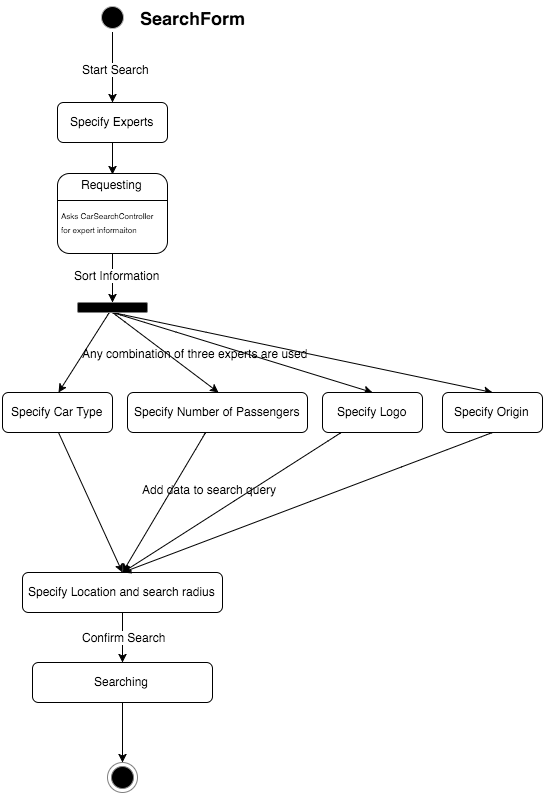
\includegraphics[scale=0.5]{searchForm-sd.png}\\

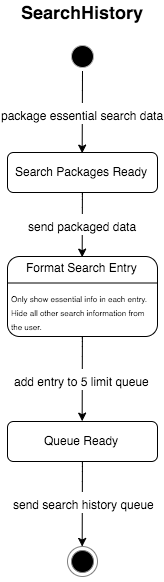
\includegraphics[scale=0.5]{searchHistory-sd.png}\\
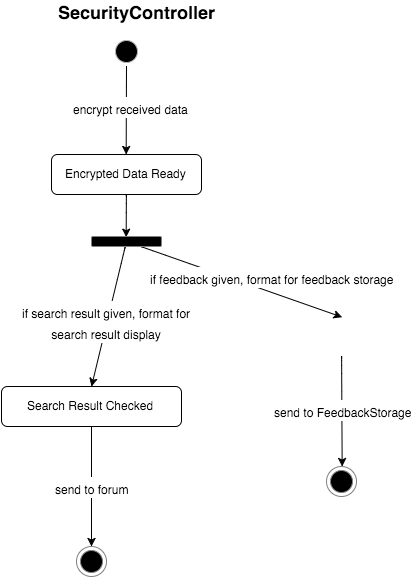
\includegraphics[scale=0.5]{securityController-sd.png}\\
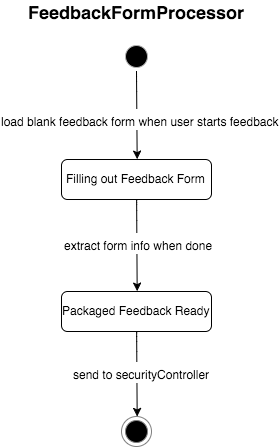
\includegraphics[scale=0.5]{feedbackFormProcessor-sd.png}\\
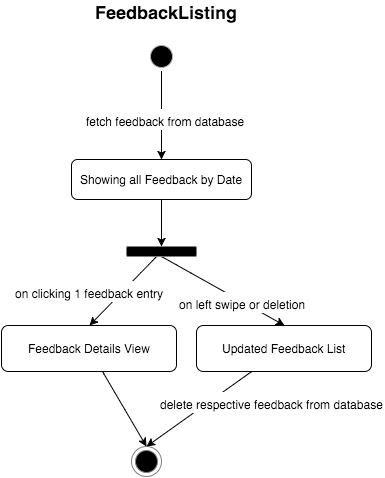
\includegraphics[scale=0.5]{feedbackListing-sd.png}\\
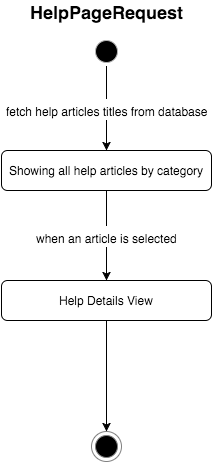
\includegraphics[scale=0.5]{helpPageRequest-sd.png}\\
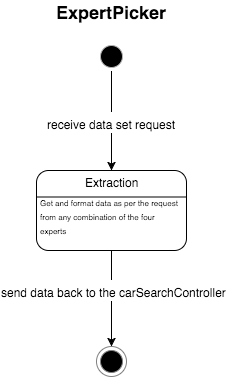
\includegraphics[scale=0.5]{expertPicker-sd.png}\\
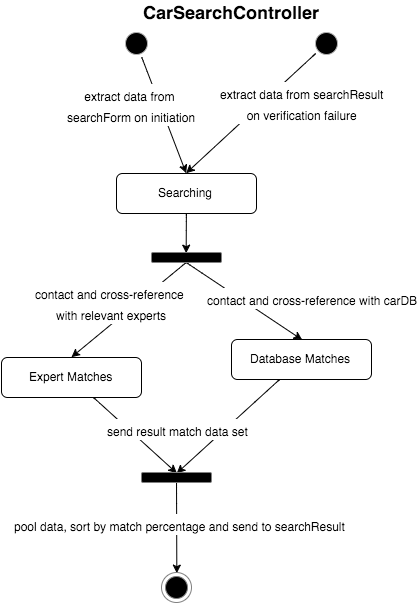
\includegraphics[scale=0.5]{carSearchController-sd.png}\\

\section{Sequence Diagrams}
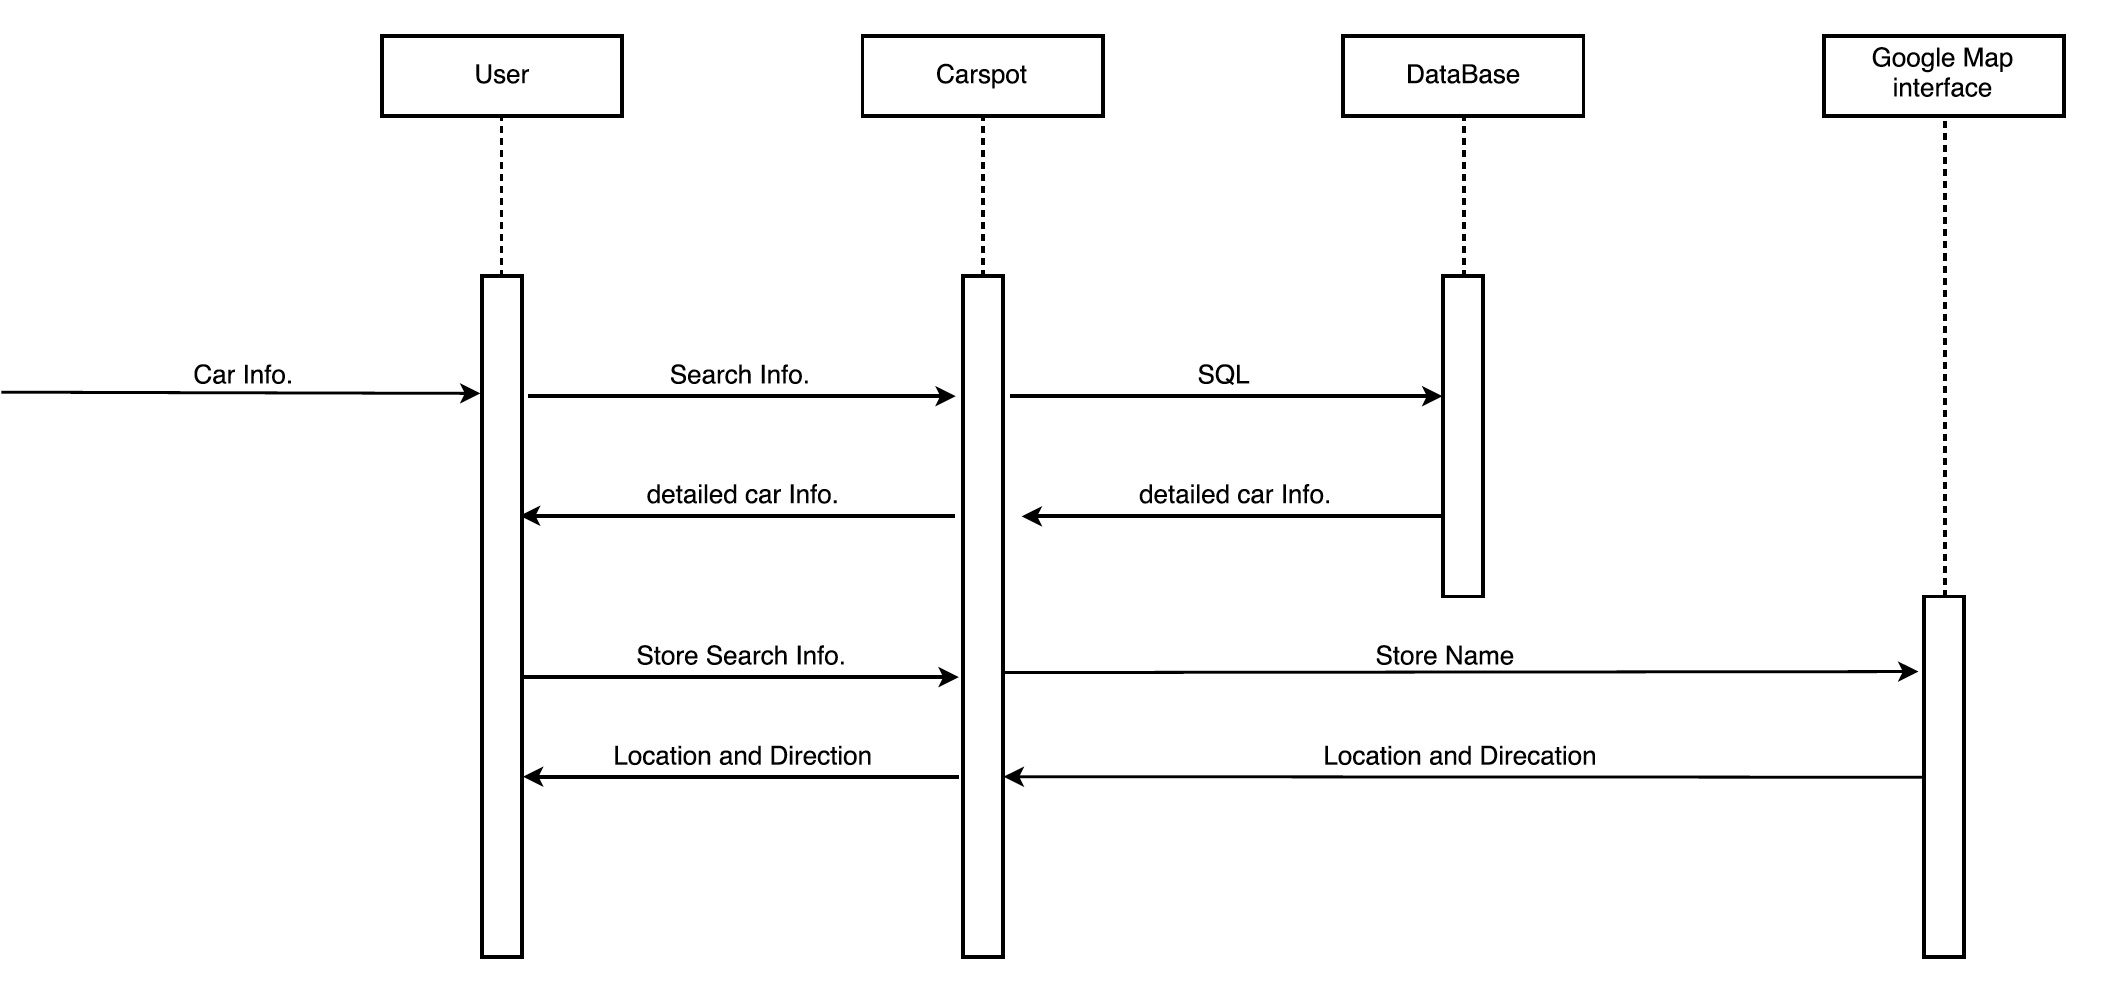
\includegraphics[width=\textwidth]{sequence.png}

\section{Detailed Class Diagram}
\includegraphics[width=\textwidth]{detailed_class.png}

\newpage

\FloatBarrier
\appendix
\section{Revision History}
\begin{table}[ht]
	\centering
	\begin{tabular}{|p{2cm}|p{5cm}|p{3cm}|p{3cm}|}
		\hline
		\textbf{Revision} & \textbf{Sections Modified} & \textbf{Date Completed} & \textbf{Contributors}\\
		\hline
	\end{tabular}
	\caption{Revision History}
	\label{table:1}
\end{table}
\section{Division of Labour}
\label{sec:division_of_labour}
% Begin Section
\begin{table}[ht]
	\centering
	\begin{tabular}{|p{2cm}|p{5cm}|p{5cm}|}
		\hline
		\textbf{Team Member:} & \textbf{Sections Completed:} & \textbf{Sections Reviewed}\\
		\hline
		Abhijit & Section 2 & Section 4\\
		\hline
		Cole & Section 4 with David's Help & Section 2\\
		\hline
		David & Section 1,4 & Section 3\\
		\hline
		Sharon & Section 3 & Section 1\\
		\hline
		Yash & Section 2 & Section 1\\
		\hline
		Yuchen & Section 3 & Section 2\\
		\hline
	\end{tabular}
	\caption{Division of Labour}
	\label{table:1}
\end{table}
% End Section

\end{document}